\documentclass[../main.tex]{subfiles}

\begin{document}

\chapter{Method}
\label{sec:sixth}

\section{Qiskit}
There are lots of available quantum computing libraries making the implementation and simulation of quantum circuits and systems easier, but the chosen one used i this thesis is qiskit\cite{Qiskit_book} which is a python library made by IBM, making it possible to simulate a q1uantum computer running a quantum circuits on a classical computer, both with and without. Write something more maybe about exact statevector simulation?idk Have a look at qiskit mentions in articles
\todo[inline]{Write more about qiskit and statevector and such, and include measurements and smaplings}

\subsection{Types of backends?}

\section{Datasets}
\subsection{Synthetic made fraud classification}
Hundreds of million transactions are completed each day around the world, which is why fraudulent transactions are so important to sieve out and eliminate, which also is a great fit for the abilities of machine learning. Even though there are lots and lots of bank transactions each day around the world, collecting a dataset in search of a complete dataset to be used to classify fraud could easily turn to a burdensome venture due to multiple reasons. First and foremost due to ethical reasons regarding stringent privacy of financial data such transaction details are not always available, in addition to labeling such data is often an overtiring process \cite{atman}. It is also worth mentioning that fraudulent bank transactions are much less likely to happen, which would give a large imbalance of fraud to non fraud categories. Lucky for us, synthetic made fraud transactions are created to mimic real life bank transactions based on \cite{atman}, which will serve as a transaction dataset in this thesis. The transaction dataset is published here \cite{padhi2021tabular}.

The dataset is based on transactions done in the US, including the following features: location based on ZIP code, time of the day the purchase was done, amount of dollars the transaction revolved around and Merchant Category Code(MCC) which is a way credit card companies defines what kind of services and goods are sold at different businesses.

When classifying the fraud dataset using the VarQBM, only one visible qubit is necessary due to transactions being either fraud or not fraud. Therefore the VarQBM will be applied to the fraud dataset using one hidden and one visible nodes in addition to the two ancilla qubits.

\subsubsection{Preprocessing the transaction dataset}
Since preprocessing of data is such an important aspect of machine learning some preprocessing will naturally be applied to the transaction data as well. Firstly the features are discretized into certain bins in resemblance with \cite{VQB:litteraturelist}. The ZIP codes are discretized and relabeled into 0,1 or 2 regarding if the ZIP code belongs to the east, central or west of the US accordingly. The time of purchase were also discretized in groups of transactions completed between, 0AM and 11AM, 11AM and 6PM and 6PM and 0AM corresponding to labels of 0,1 and 2 accordingly. The same were done for amounts less than \$50, between \$50 and 150, and more than \$150, into bins labeled 0,1 and 2 accordingly. The remaining discretization were applied to the MCCs. By studying MCCs with values less than 10.000, opens up the door of splitting the MCC feature into 10 more features containing 0's and a 1, according to the thousandth of the MCC.
\todo[inline]{Maybe use a table instead to show the discretization}

The datasets used consists of three sets, a training set consisting of 500 samples. A validation set, consisting of 250 samples which will be used to explore the optimal amount of training epochs needed to minimize the validation loss and prevent overfitting and underfitting. And a test set to see how well the final model generalizes. Each of the three sets contains 20\% fraudulent credit card transactions, which is more in terms with real world transactions, due to most transactions in real life being non-fraudulent. The data is also scaled by applying standardization to the features to ensure a centered mean and unit-variance.

\subsection{Handwritten digits}
The next datasets used in the thesis were based on classifying handwritten digits based on images or pixel strengths in other words. Both a smaller digit dataset made by \cite{UCI_repo2019} containing approximately 180 samples of each digit collected from a total of 43 people with sample sizes of 8 x 8 pixels, the dataset will be referred to as the 'digit dataset' in the thesis. The other dataset based on handwritten digits used is the more advanced and famous MNIST dataset\cite{deng2012mnist} which is one of the most popular datasets within machine learning and a remarkable way of testing new machine learning models. The MNIST dataset consists of more than 60.000 training samples in addition to a 10.000 sized test set. The size of the samples are 28 x 28 pixels. This dataset will be referred to as the 'MNIST dataset' in the thesis.

To keep the computational time and number of circuits in addition to run enough epochs to train a complete model only four classes will be used. Using only samples from four classes makes it possible to classify the four numbers of the digits datasets using only 2 visible qubits and 2 ancilla qubits.

\subsubsection{Preprocessing of handwritten digit datasets}
Due to the limited number of samples, in the digit dataset, the sets used will only consist of a train set and a validation set-which will behave as a test set. Following the trend from the transaction dataset, the training sets for both handwritten datasets will use training sets containing 500 samples. The digit dataset will use the rest of available data as a validation set, while the MNIST dataset will use a validation- and a test set of 250 samples each.

Scaling the data is always a clever idea, and due to pixel values in images having values in the range of $[0,255]$, it is quiet typical to scale images using min-max normalisation to ensure feature values between in the range of $[0,1]$, which will be done on both handwritten datasets. Further more the pixels will 

\subsection{Franke's function}
Franke's function is often used as a function to test different regression methods. Franke's function is a three dimensional function which can be seen in figure \autoref{fig:frankesplot}. Franke's function has two Gaussian peaks of differing heights, and a smaller dip. The formula of the function goes as follows:

\begin{align*}
\begin{split}
  f(x,y) &= \frac{3}{4}\exp{\left(-\frac{(9x-2)^2}{4} - \frac{(9y-2)^2}{4}\right)}+\frac{3}{4}\exp{\left(-\frac{(9x+1)^2}{49}- \frac{(9y+1)}{10}\right)} \\
  &+\frac{1}{2}\exp{\left(-\frac{(9x-7)^2}{4} - \frac{(9y-3)^2}{4}\right)} -\frac{1}{5}\exp{\left(-(9x-4)^2 - (9y-7)^2\right)}
\end{split}
  \label{eq:franke-func}
\end{align*}

\begin{figure}[ht]
    \begin{center}
        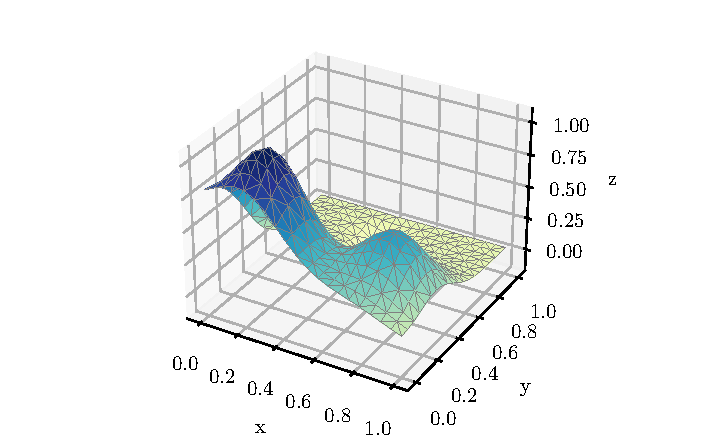
\includegraphics{figures/real_franke.pdf}
        \caption{Shape of Franke's function which will be used as a regression goal.}
        \label{fig:frankesplot}
    \end{center}
\end{figure}

\subsubsection{Using the Vandermonde matrix to sort data from Franke's function}
Keeping data in a well designed system for easy access and application is important in all sorts of supervised learning tasks. Due to sampling probabilities of qubits in quantum computations being quiet unstable leaving lots of room for deviations, Franke's data are sorted into a so called Vandermonde matrix containing geometrical progression of the data, and used as a design matrix. The design matrix is constructed by creating each sample as a polynomial of some x and y point extracted from Franke's function the following way:

\begin{equation*}
\mathbf X=  \begin{pmatrix}
   1& x_0 & y_0 & x_0^2 & x_0y_0 & y_0^2 & \ldots & x_0^d y_0^{d}\\
    1& x_1 & y_1 & x_1^2 & x_1y_1 & y_1^2 & \ldots & x_1^d y_1^{d}\\
    & &  &  &  &  & \vdots & \\
    1 & x_{n} & y_{n} & x_{n}^2 & x_{n}y_{n} & y_{n}^2 & \ldots & x_{n}^d y_{n}^{p}\\
 \end{pmatrix}
\end{equation*}

With $d$ being the degree of polynomial. Making the degree higher leads to more complicated equations which naturally gives a more precise fit to the training data, and therefore increasing the possibility of overfitting. It is worth mentioning that by using a polynomial Vandermonde matrix will lead to some correlation between the samples, but since the goal of using the mentioned dataset is to see how well the VarQBM are able to manipulate sampling probabilities in regression and study how well this can be generalized, a blind eye will be turned towards the correlating part of the samples.

\subsubsection{Preprocessing and generation of the Franke data}
When generating the dataset some stochastic noise \ensuremath{\epsilon\sim\mathcal{N}(0,\sigma)} are also added to Franke's function as an effort to lessen the chance of overfitting. The data is generated by inserting equally spaced points as \ensuremath{x,y \in [0,1]} together with the desired degree of polynomial into the aforementioned design matrix which is created and filled with values from Franke's function.

The values are already quiet nicely lined up due to \ensuremath{x,y \in [0,1]}, but to ensure that the target variable also lays between $0$ and $1$ min-max normalisation is applied to Franke's data. This is crucial to have all target variables lay in the span of possible sampling probabilities. The data used consists of $20x20=400$ samples which is divided into a train- and validation/test with a ration of $0.75$ and $0.25$ accordingly. The chosen degree of polynomial is $5$ to keep the correlations and overfitting within a reasonable level, which gives 21 features.

\section{Variational Quantum Boltzmann machine}
\todo[inline]{Explains a general outline on how the VarQBM is initialised, and explain different aspects of it under}
The VarQBM primarily consists of three steps. The initialisation and optimization of Hamiltonian coefficients in addition to preparing a trial circuit which yields Bell states when subtracing pairwise qubits of the trial circuit. Generating and preparing Gibbs states, and finally computing the Boltzmann distribution and derivatives which is nedded for the optimization process.

After the Hamiltonian and the trial circuit are ready to go, the circuits are sent into the varITE class, which prepares the Gibbs states of the circuits, and the corresponding derivatives. The Gibbs states are then used to compute the Boltzmann distribution along with the gradient of the Boltzmann distribution with respect to the Hamiltonian parameters, using the chain rule along with the derivatives of the Gibbs states. The gradients are then used to optimize the coefficients of the Hamiltonian according to some optimization technique to reproduce some specific target distribution. This naturally goes on for multiple loops, until the optimal parameters are found.

\subsection{Initialisation of Hamiltonian coefficients}
When doing generative learning, generating target probability distributions, the Hamiltonian coefficients are drawn from an uniform distribution from the interval of $[-1, 1]$ in accordance with \cite{VQB:litteraturelist}.

When doing discriminative learning, the input of samples must to be encoded into the VarQBM. This is done using two approaches, first approach is done by following the bias dot product method explained in \autoref{sec:bias_dot_product}, the Hamiltonian vector which is multiplied by feature values are drawn from a uniform distribution the same way as for generative learning.
\todo[inline]{Add the referral above}

The second approach is by having feature values of a given sample encoded into the coefficients by inserting them into a DNN, which goes through the network and outputs the Hamiltonian coefficient. 

\subsubsection{Neural network to initialise the Hamiltonian}
When initiating a DNN there are multiple parameters that affects the initialisation and thereby the output. Firstly the weights and bias of the network need to be initialised, there are lots of different ways to do this, but in this thesis Xavier normal- and uniform and He normal- and uniform will be explored.

In addition activation functions are most often favoured to include in a neural network. Some different activation functions are tested to observe the rate of convergence toward some minimum. An overview of the activation functions used in this thesis can be seen in \autoref{tab:activaton_functions}

\begin{table}[h!]
\centering
\caption{A variety of activation functions used common in neural networks}
\begin{tabular}{c c} 
\hline
Name  & Activation Function \\
\hline
Identity  & $f(x)=x$ \\
Sigmoid  & $f(x)=\frac{1}{(1+e^{-x})}$ \\
Tanh  & $f(x)=\frac{e^x-e^{-x}}{e^x+e^{-x}} $ \\
Leaky Relu  & $f(x)=\max(0.01x, x)$ \\
\end{tabular}
\label{tab:activaton_functions}
\end{table}

Another thing is probably is one of the most important things to define in a neural network is the number of layers and hidden nodes within each layers. Therefore multiple sizes of layers will be tested, in addition to putting the very rough general rule of thumb called the pyramid rule provided in \cite[ch.~10]{Timothy_Masters} to test. The pyramid rule is a quiet shallow direction of choosing the size of neural networks consisting of one or two layers. The rule is based on creating a pyramid shaped network, in other words having the input layer stand as the largest layer in the network, followed by a smaller hidden layer, which goes on until the output layer consisting of the fewest nodes are reached. 

The geometric progression of hidden nodes in a 1- hidden layer network consists of $\sqrt{mn}$, with $n$ being the number of input neurons and $m$ corresponding to the output neurons.

A 2-hidden layer network would have a quiet similar approach by defining a variable $r=\sqrt[3]{\frac{n}{m}}$, which gives the following hidden layer sizes:
\begin{align*}
    NHid_1=&mr^2\\
    NHid_2=&mr
\end{align*}

Eventhough the pyramid rule only should be used as a guideline of the network sizes, this should be sufficient in this particular case due to the network only being used to find Hamiltonian coefficients used in the VarQBM, the heavy lifting is still executed by the VarQBM, which gives room for the neural network not necessarily using the most optimal parameters. 

\subsection{Variational imaginary time evolution}
The preparation of Gibbs states through VarITE is one of the main parts of the VarQBM. After inserting the trial circuit and the Hamiltonian into the VarQITE class, all circuits needed are created before the time evolution starts. Since the parameters evolved through varITE are the parameters of the trial circuit, all circuits can be initialized before the time evolution starts, and bind new parameters to the gates after each timestep.

The initial trial circuit $V(\omega(0))$ are sent into the VarITE process with the objective of computing $\omega(\tau)$ and the corresponding derivative $\frac{\partial \omega(\tau)}{\partial \theta}$ with $\tau$ being the final time. When the time evolution starts off, matrix $A(t)$ and vector $C(t)$ are computed according to \autoref{sec:VarITE} at time step $t$. Which are then put together as a system of equations $A(t)\dot{\omega}=C(t)$, which results in the derivative of the trial circuit parameters with respect to current time step. Due to matrix $A(t)$ having a possibility of being singular, hence having infinite many solutions, non-invertible matrices are more probable to make an appearance when the trial circuit consists of an excessive amount of symmetry. Dealing with ill-conditioned systems of equations are done by applying Ridge or Lasso regression to the system. The regularizing term should be small enough to ensure that matrix $A$ is invertible or tuned to give the least amount of difference between $A\dot{\omega}$ and $C(t)$.

Further on a loop goes through each of the Hamiltonian parameters, computing the derivative of $\omega(t)$ with respect to the Hamiltonian coefficients. This is done using regularization schemes as done earlier in the VarITE process. After each time step $\omega$ and $\frac{\partial\omega}{\partial \theta}$ are updated using explicit Euler methods. An outline of the algorithm from \cite{VQB:litteraturelist} can be seen in \autoref{algo:VarQITE}

\begin{algorithm}[ht]
 \caption{VarQITE for \varqbm} \label{algo:VarQITE}
\begin{algorithmic}[0]
    \State  \textbf{input}
    \State $H_{\text{eff}} = H_{\theta}^a + I^b$
	\State$\tau = {1}/{2\left(\text{k}_{\text{B}}\text{T}\right)}$
	\State $\ket{\psi\left( \omega\left(0\right)\right)} = V\left(\omega\left(0\right)\right)\ket{0}^{\otimes 2n} = \ket{\phi^{+}}^{\otimes n}$
	\State with $\ket{\phi^{+}} = \left(\ket{00}+\ket{11}\right)/{\sqrt{2}}$
    \State \textbf{procedure}
	\For{$t\in\set{\delta\tau, 2\delta\tau, \ldots, \tau}$}
		\State Evaluate $A\left(t\right)$ and $C\left(t\right)$
		\State Solve $A\dot{\omega}\left(t\right) = C$
		\For{$i\in\set{0, \ldots, p-1}$}
    			\State Evaluate $\partial_{\theta_i}C$ and $\partial_{\theta_i}A$
    			\State \label{item:linEqDer}Solve $A\left(\partial_{\theta_i}\dot{\omega}\left(t\right)\right)  = \partial_{\theta_i}C - \left(\partial_{\theta_i}A\right)\dot{\omega}\left(t\right)$
    			\State \label{item:grad_omega_tau}Compute $ \: \partial_{\theta_i}{\omega}\left(t+\delta\tau\right) = \partial_{\theta_i}{\omega}\left(t\right)+\partial_{\theta_i}\dot{\omega}\left(t\right)\delta\tau$
	   \EndFor
		\State \label{item:computeUpdateDer}Compute $\omega\left(t+\delta\tau\right) = \omega\left(t\right) +   \dot{\omega}\left(t\right)\delta\tau $
	\EndFor
	\State \textbf{return} $\omega\left(\tau\right), \: \partial\omega\left(\tau\right)/\partial\theta$
\end{algorithmic}
\end{algorithm}

\subsubsection{Computing- and interpreting the Boltzmann distribution to classification- and regression values}
After finding the Gibbs states from the VarITE process, tracing out the ancillary system, the Boltzmann distribution are then found by doing a projective measurement on the quantum states representing the visible qubits for each possible configuration of the visible qubits, which would translate to the diagonal of the matrix corresponding to the visible qubits.

Translating the Boltzmann distribution into classification values are quiet easily done by. When doing multiclass labeling, the Boltzmann distribution is used as a one hot encoded vector, meaning that the each index of the distribution represents one label, giving the index of largest probability the final label. In multilabel classification the needed number of visible qubits $n$ scales exponential with the number of classes $2^n$. When doing binary classification, only one visible qubit is needed, interpreting the probability of the qubit being in state 0 or 1 as the probability of the binary label being 0 or 1. Regression problems follow the same lane, using the sampling probability as the regression values, ensuring that the true values are scaled within 0 and 1.

\subsection{Optimization process}
The optimization process of the VarQBM is conducted in a classical fashion without the use of quantum algorithms. The optimization process is quiet usual compared to most optimization problems. The loss function used throughout the thesis is primarily cross entropy, with an exception of MSE used with regression of Franke's function. Due to the sampling probability being a regression target instead of a probability distribution.

After a prediction is done within the VarQBM, the gradients of the probabilities corresponding to each configuration is computed using the parameter shift rule introduced in section \ref{sec:parameter_shift}. The derivatives are taken further to compute the gradients of the loss with respect to each Hamiltonian parameter. Now all the necessary gradients are computed and are used to optimize the Hamiltonian according to some optimizer. Multiple optimizers will be tested to evaluate how the choice of optimization technique affects the Boltzmann distribution. Due to the relatively high number of circuits simulated when doing an iteration of VarITE, some form of SGD optimization is executed

\todo[inline]{Add referral to the parameter shift rule, is it even necessary to refer to the theory section?}

\section{Restricted Boltzmann machine}
When referring to a classical Boltzmann machine or a RBM in this thesis, a classical computational approach is taken without the use of quantum algorithm. Due to problems of convergence well known when using regular Boltzmann machines, the classical approaches of Boltzmann machines in this thesis is therefore done utilizing RBMs. Two classical RBMs are utilized in this thesis, a Bernouilli-RBM and a Gaussian-binary RBM.

\subsection{Scikit learn's Bernoulli-RBM}
A Bernoulli-RBM provided by the widely used python library Scikit Learn\cite{scikitlearn} is used when doing classification- and regression tasks on classical datasets. A Bernoulli-RBM originally only accepts binary nodes for both visible and hidden nodes, but by inserting  real valued visible values in the range of $[0,1]$ instead, the visible states are treated as visible probabilities instead of binary states, the scikit learn class automatically initialises the variance as $0.01$ prior to the training. Therefore data applied to  accepting real valued input, therefore the data are scaled in the 

\subsection{Gaussian-Binary RBM}
When utilizing a classical RBM to solve a quantum mechanical problem, a self written Gaussian-Binary RBM using a Variational Monte Carlo approach is implemented using C++.

\subsection{Modelling the Hydrogen system}
The hydrogen system consists of two hydrogen atoms at fixed positions with distance $R$ between them. The modell can be seen in \autoref{fig:h2model}

\begin{figure}[ht]
    \begin{center}
        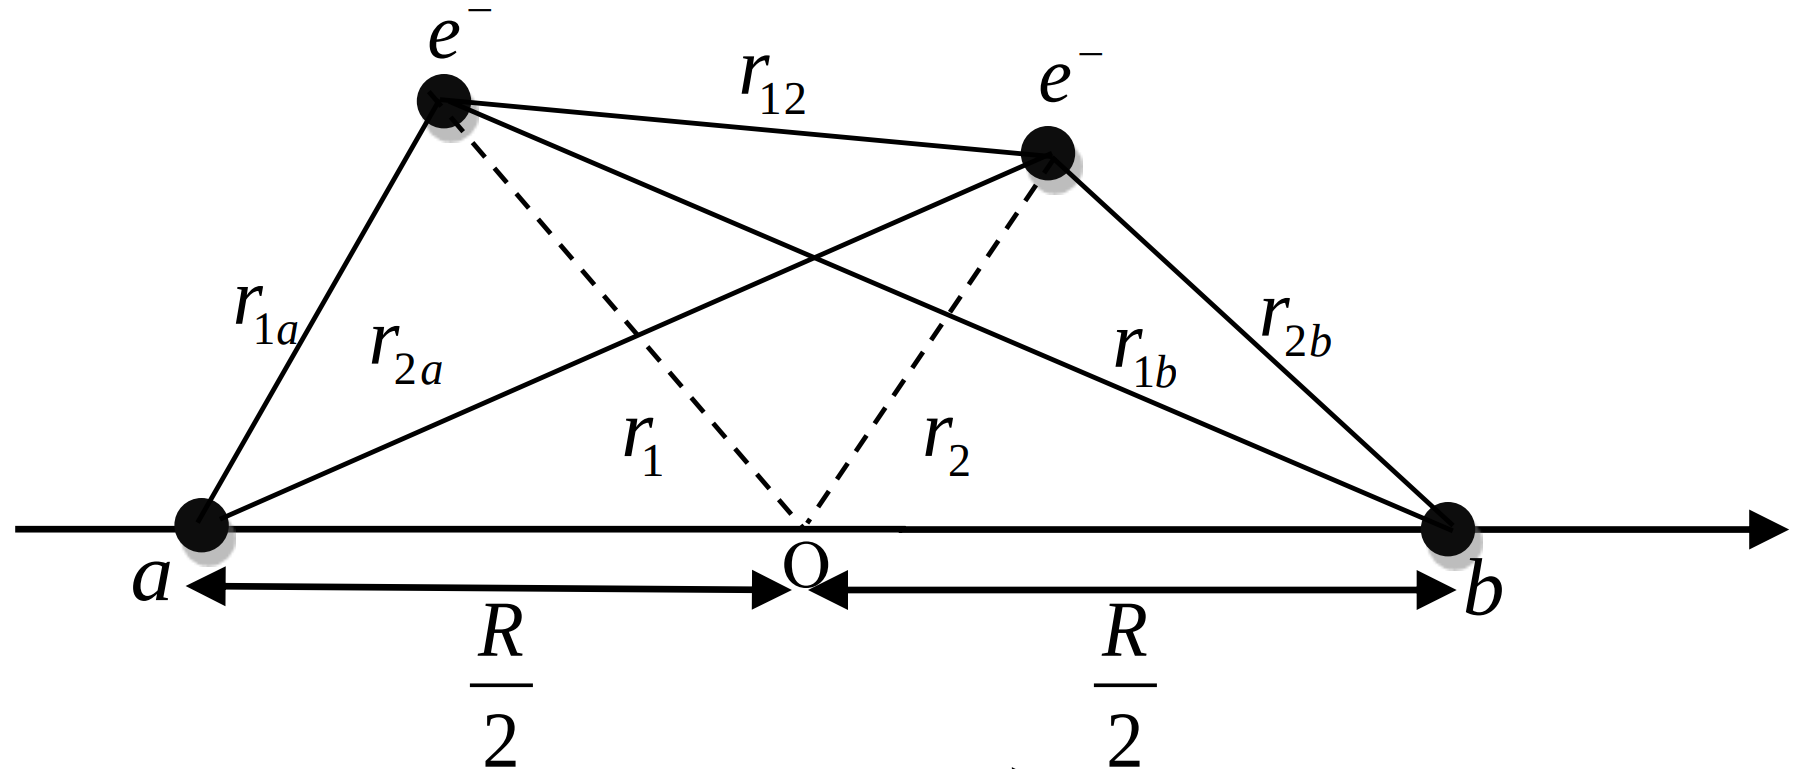
\includegraphics[scale=0.15]{figures/perfect.png}
        \caption{H2 model. Figure from \cite{hydrogen_model_figure}}
        \label{fig:h2model}
    \end{center}
\end{figure}

\subsubsection{Implementation of the Gaussian RBM}
\todo[inline]{Method of RBM from fys4411, write after it is used}



\end{document}